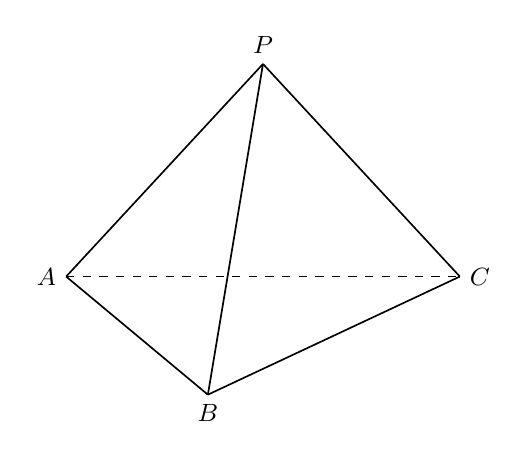
\begin{tikzpicture}[line width=0.6pt, font=\small]
\coordinate (P) at (2.5,4.2);
\coordinate (A) at (0,1.5);
\coordinate (C) at (5,1.5);
\coordinate (B) at (1.8,0);
% hidden base edge
\draw[dashed] (A) -- (C);
% visible edges
\draw (P) -- (A);
\draw (P) -- (C);
\draw (P) -- (B);
\draw (A) -- (B);
\draw (B) -- (C);
\node[above] at (P) {$P$};
\node[left] at (A) {$A$};
\node[right] at (C) {$C$};
\node[below] at (B) {$B$};
\end{tikzpicture}
